%#Region Includes & Defines
\documentclass[
	% -- opções da classe memoir --
	12pt,				% tamanho da fonte
	openright,			% capítulos começam em pág ímpar (insere página vazia caso preciso)
	twoside,			% para impressão em verso e anverso. Oposto a oneside
	a4paper,			% tamanho do papel. 
	% -- opções da classe abntex2 --
	%chapter=TITLE,		% títulos de capítulos convertidos em letras maiúsculas
	%section=TITLE,		% títulos de seções convertidos em letras maiúsculas
	%subsection=TITLE,	% títulos de subseções convertidos em letras maiúsculas
	%subsubsection=TITLE,% títulos de subsubseções convertidos em letras maiúsculas
	% -- opções do pacote babel --
	english,			% idioma adicional para hifenização
	french,				% idioma adicional para hifenização
	spanish,			% idioma adicional para hifenização
	brazil,				% o último idioma é o principal do documento
	]{abntex2}


% ---
% PACOTES
% ---

% ---
% Pacotes fundamentais 
% ---
% \usepackage{cmap}			% Mapear caracteres especiais no PDF
\usepackage{lmodern}			% Usa a fonte Latin Modern			
\usepackage[T1]{fontenc}		% Seleção de códigos de fonte.
\usepackage[utf8]{inputenc}		% Codificação do documento (conversão automática dos acentos)
% \usepackage{lastpage}			% Usado pela Ficha catalográfica
\usepackage{indentfirst}		% Indenta o primeiro parágrafo de cada seção.
\usepackage{color}				% Controle das cores
\usepackage{graphicx}
\usepackage{float}
\usepackage{enumitem}
\usepackage{mathtools}
\usepackage{pdflscape}
\usepackage{textcomp}
% ---
		
% ---
% Pacotes adicionais, usados apenas no âmbito do Modelo Canônico do abnteX2
% ---
% \usepackage{lipsum}			% para geração de dummy text
% ---

% ---
% Pacotes de citações
% ---
\usepackage[brazilian,hyperpageref]{backref}   % Paginas com as citações na bibl
\usepackage[alf]{abntex2cite}	                         % Citações padrão ABNT

% --- 
% CONFIGURAÇÕES DE PACOTES
% --- 

% ---
% Configurações do pacote backref
% Usado sem a opção hyperpageref de backref
\renewcommand{\backrefpagesname}{Citado na(s) página(s):~}
% Texto padrão antes do número das páginas
\renewcommand{\backref}{}
% Define os textos da citação
\renewcommand*{\backrefalt}[4]{
	\ifcase #1 %
		Nenhuma citação no texto.%
	\or
		Citado na página #2.%
	\else
		Citado #1 vezes nas páginas #2.%
	\fi}%
% ---
%#Endregion

%#Region Informações de capa
% ---
% Informações de dados para CAPA e FOLHA DE ROSTO
% ---
\titulo{}
\autor{Francisco Gomes Soares Sanches Manso}
\local{Belo Horizonte}
\data{\today}
\orientador[Orientador:]{Dalton Martini Colombo}
% \coorientador[Coorientador:]{}
\instituicao{%
  Universidade Federal de Minas Gerais -- UFMG
  \par
  Escola de Engenharia
  \par
  Programa de Pós-Graduação em Engenharia Elétrica}
\tipotrabalho{Dissertação de Mestrado}

% O preambulo deve conter o tipo do trabalho, o objetivo, o nome da instituição e a área de concentração 
\preambulo{Dissertação submetida ao Programa de Pós-Graduação em Engenharia Elétrica da Universidade Federal de Minas Gerias, como parte dos requisitos necessários à obtenção do título de Mestre em Engenharia Elétrica.}
% ---

% ---
% Configurações de aparência do PDF final

% alterando o aspecto da cor azul
\definecolor{blue}{RGB}{41,5,195}

% informações do PDF
\makeatletter
\hypersetup{
     	%pagebackref=true,
		pdftitle={\@title}, 
		pdfauthor={\@author},
    	pdfsubject={\imprimirpreambulo},
	    pdfcreator={LaTeX with abnTeX2},
		pdfkeywords={abnt}{latex}{abntex}{abntex2}{trabalho acadêmico}, 
		colorlinks=true,       	% false: boxed links; true: colored links
    	linkcolor=blue,          	           % color of internal links
    	citecolor=blue,        		% color of links to bibliography
    	filecolor=magenta,      		% color of file links
		urlcolor=blue,
		bookmarksdepth=4
}
\makeatother
% --- 

% --- 
% Espaçamentos entre linhas e parágrafos 
% --- 

% O tamanho do parágrafo é dado por:
\setlength{\parindent}{1.3cm}

% Controle do espaçamento entre um parágrafo e outro:
\setlength{\parskip}{0.2cm}  % tente também \onelineskip

% ---
% compila o índice
% ---
\makeindex
% ---

% ----
% Início do documento
% ----
\begin{document}

% Retira espaço extra obsoleto entre as frases.
\frenchspacing 

% ----------------------------------------------------------
% ELEMENTOS PRÉ-TEXTUAIS
% ----------------------------------------------------------
% \pretextual

% ---
% Capa
% ---
\imprimircapa
% ---

% ---
% Folha de rosto
% ---
\imprimirfolhaderosto
% ---

% ---
% Dedicatória
% ---
% \begin{dedicatoria}
%    \vspace*{\fill}
%    \centering
%    \noindent
%    \textit{.} \vspace*{\fill}
% \end{dedicatoria}
% ---

% ---
% Agradecimentos
% ---
% \begin{agradecimentos}
% .
% \end{agradecimentos}
% ---

% ---
% Epígrafe
% ---
% \begin{epigrafe}
%     \vspace*{\fill}
% 	\begin{flushright}
% 		\textit{.}
% 	\end{flushright}
% \end{epigrafe}
% ---
%#Endregion

%#Region Resumos & Listas
% ---
% RESUMOS
% ---
% resumo em português
\setlength{\absparsep}{18pt} % ajusta o espaçamento dos parágrafos do resumo
\begin{resumo}
	

	\vspace{\onelineskip}

	\noindent 
	\textbf{Palavras-Chave}: Palavras-chave
\end{resumo}

% resumo em inglês
\begin{resumo}[Abstract]
	\begin{otherlanguage*}{english}
		

		\vspace{\onelineskip}
		
		\noindent 
		\textbf{Key-words}: Key-words.
	\end{otherlanguage*}
\end{resumo}

% ---
% inserir lista de ilustrações
% ---
\pdfbookmark[0]{\listfigurename}{lof}
\listoffigures*
\cleardoublepage
% ---

% ---
% inserir lista de tabelas
% ---
% \pdfbookmark[0]{\listtablename}{lot}
% \listoftables*
% \cleardoublepage
% ---

% ---
% inserir lista de abreviaturas e siglas
% ---
\begin{siglas}
	\item[ADC] Analog to Digital Converter
	\item[DAC] Digital to Analog Converter
	\item[VTC] Voltage to Time Converter
	\item[VCDU] Voltage Controlled Delay Unit
\end{siglas}
% ---

% ---
% inserir lista de símbolos
% ---
\begin{simbolos}
  \item[$ f_{s} $] Frequência de amostragem
\end{simbolos}
---

% ---
% inserir o sumario
% ---
\pdfbookmark[0]{\contentsname}{toc}
\tableofcontents*
\cleardoublepage
% ---

% ----------------------------------------------------------
% ELEMENTOS TEXTUAIS
% ----------------------------------------------------------
\textual

%#Endregion

% ----------------------------------------------------------
%#Region Capítulo 1 - Introdução
% ----------------------------------------------------------
\chapter{Introdução}

%#Endregion

% ----------------------------------------------------------
%#Region Capítulo 2 - Revisão Bibliográfica
% ----------------------------------------------------------

\chapter{Revisão Bibliográfica}
	
	(Essa primeira parte eu fiz mais como um brainstorm pra guiar meu pensamento. Provavelmente não está organizada de maneira ideal e possívelmente parte é desnecessária)

	A realização de operações matemáticas de dois sinais ou de duas variáveis são comumente calculadas ou no domínio de sinais analógicos ou no domínio dos sinais digitais. Cada domínio oferece uma vantagens e desvantagens que podem ser melhor aproveitadas em situações específicas. Em ambos casos, operações matemáticas podem ser implementadas por circuitos elétricos.

    Um exemplo de operações matemáticas no domínio analógicos é recorrente nos filtros analógicos. Os filtros analógicos são comumente empregados nos filtros anti-aliasing. Tais circuitos são em geral utilizados para remover as frequências mais altas, fora da região de interesse, de um dado sinal de entrada. A importância desses filtros se baseia na preservação do Teorema da Amostragem, a fim de respeitar a frequência de Nyquist\cite{nyquist}.

    A filtragem de um dado valor pode ser modelado como a convolução deste sinal no tempo com uma $sinc$ com amplitude e frequência específicas. A convolução, por sua vez, nada mais é que a integral de um produto\cite{Oppenheim}.
	
	$$y(t)=\int_{-\infty}^{+\infty} f(t)g(x-t)dt=f(t)*g(t)$$

    De maneira análoga, têm-se os filtros do domínio digital. Os chamados filtros de reconstrução são utilizados para converter um dado sinal amostrado em uma forma de onda fidedígna às frequências amostradas. Esse filtro é implementado na versão discreta da filtragem analógica\cite{Oppenheim}.

	$$x_r(t)=\sum_{n=-\infty}^{+\infty} x[n]h_r(t-nT)$$
	$$h_r(t)=sinc(\pi t f_s)$$

    Na equação acima, fica evidente como duas operações fundamentais como o produto e a soma podem ser utilizadas para implementar filtros e operações elaboradas entre sinais.

	Em tecnologias mais recentes, há uma escalada em direção à miniaturização dos sistemas e suas unidades de processamento\cite{kuo}. Muitas vezes essa miniaturização é refletida na redução da escala dos componentes fundamentais dos sistemas analógicos e digitais: os transistores. Uma das características mais salientes da redução do comprimento do canal de um transistor de efeito de campo é a redução da tensão de ruptura do semicondutor\cite{Sze}. Por consequência, faz-se necessária a redução da tensão de operação do dispositivo a fim de evitar o estresse do transistor\cite{kuo}.

	Tecnologias que utilizam tensão de operação reduzida tendem a dificultar a manutenção de uma boa relação sinal-ruído de sinais analógicos. Com a tensão de operação reduzida, há uma redução na faixa de excursão do sinal, mas não necessariamente uma redução na amplitude do ruído. Os sistemas analógicos não vêm conseguindo acompanhar a escalada das tecnologias no mesmo passo: com a redução cada vez maior dos níveis de operação, manter uma boa relação sinal-ruído têm-se tornado um desafio. \cite{kuo}

    Por muitas vezes, faz-se necessário a interface entre os domínios analógicos e digital de tal forma que é necessário uma conversão entre as grandezas discretas e contínuas. Alguns conversores são utilizados para tais situações, como os conversores analógico-digital (\textit{Analog to Digital Converter} - ADC) e os conversores digital-analógico (\textit{Digital Analog Converter} - DAC). Tais conversores atuam no sentido converter grandezas entre os domínios analógico e digital, em que o primeiro é naturalmente contínuo em tempo e amplitude de tensão, e o segundo é discreto tanto em tempo quanto em amplitude de tensão. Apesar das diferenças entre os domínios, ambos utilizam a amplitude de tensão como meio de representar a informação. Podemos assim dizer que ambos domínios analógico e digital estão inseridos no \textbf{domínio tensão}.(fonte?)

	Dessa forma, pode-se utilizar um \textbf{conversor tensão-tempo} (\textit{Voltage to Time Converter} - VTC), para converter tanto um sinal analógico quanto um sinal digital para o domínio do tempo. Já o caminho inverso é bifurcado, podendo-se converter um signal no domínio tempo tanto para analógico, utilizando um conversor tempo-analógico (), quanto para digital, utilizando um conversor tempo-digital \textit{Time to Digital Converter} - TDC).

	\section{Conversores tensão-tempo}

		Os VTCs \textbf{mapeiam} uma dada amplitude de tensão de entrada em um intervalo de tempo de saída relativo. Esse mapeamento pode ser interpretado como a conversão de um sinal no \textbf{domínio tensão} para um sinal no \textbf{domínio tempo}. Seja um sinal de entrada com amplitude de tensão $t_{in}$ e o tempo relativo entre dois eventos que mapeiam a tensão de entrada $t_{delay}$, a relação entre tais grandezas pode ser expressa por um ganho $G_{\phi}$\cite{Shivani}. Um VTC ideal relaciona de maneira linear ambas grandezas conforme abaixo.

		$$t_{delay}=G_{\phi}v_{in}$$

		Assim como os conversores ADC e DAC, os VTCs também possuem um período de tempo em que o sinal a ser convertido será amostrado, denominado de tempo de amostragem (\textit{sampling time}) $t_s$, para que seja realizada a conversão de uma grandeza em outra, denominado tempo de conversão (\textit{conversion time}) $t_c$. O $t_{delay}$ pode ter definição variada dependendo do VTC utilizado. A Figura~\ref{fig:VTC} abaixo exemplifica a conversão de um dado sinal de entrada no domínio tensão em um sinal de saída no domínio tempo.

		\begin{figure}[!ht]
			\centering
			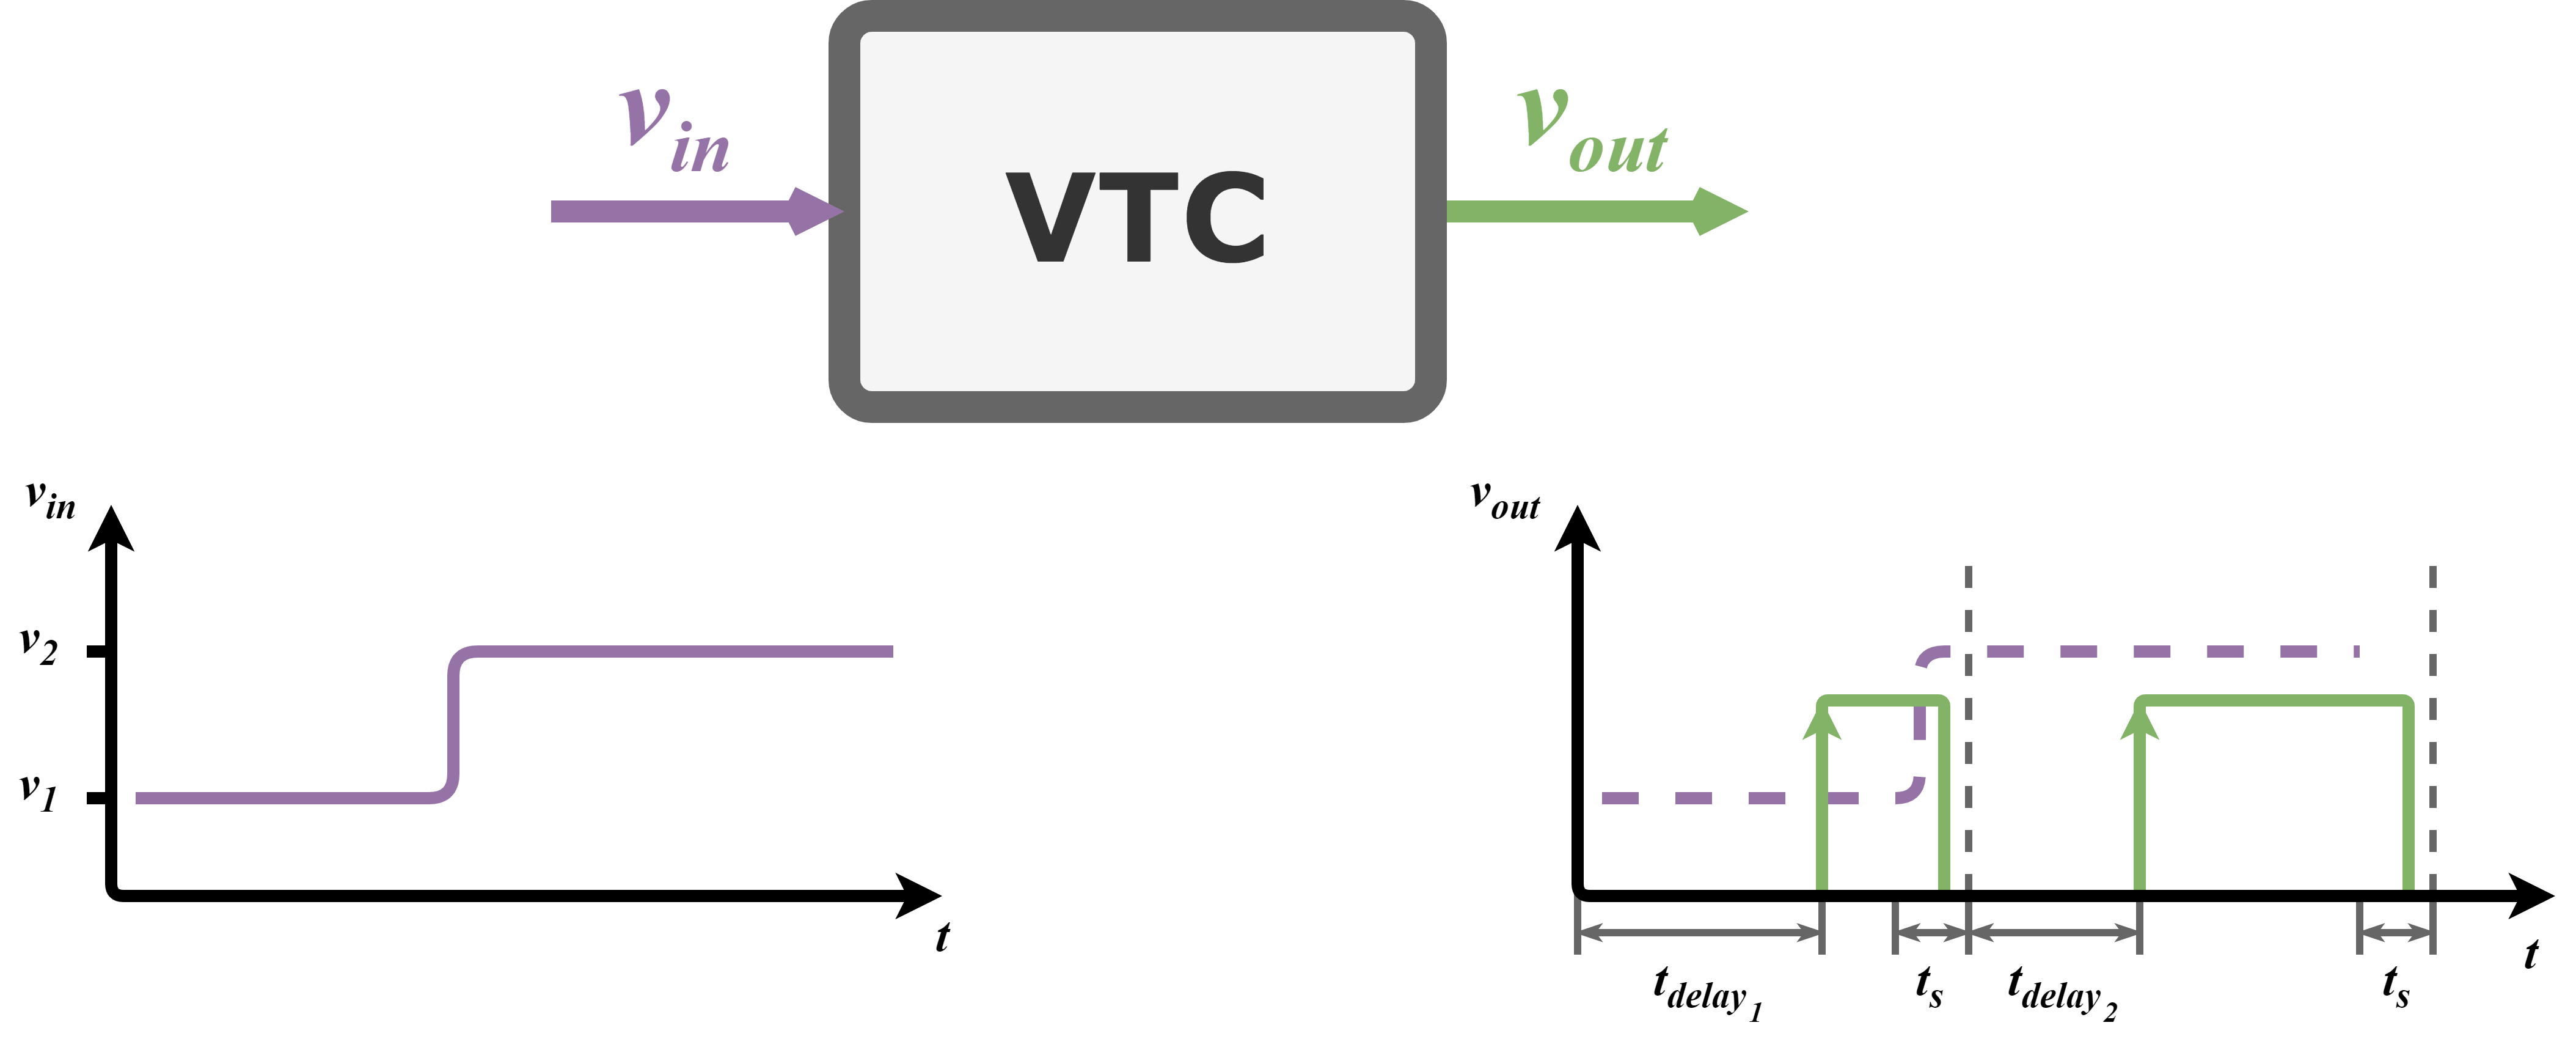
\includegraphics[width=\linewidth*3/4]{images/VTC.png}
			\caption{Exemplo de Conversor Tensão-Tempo - VTC}
			\label{fig:VTC}
		\end{figure}
		
		Nesse exemplo, a variável de tempo $t_{delay}$ é associada ao tempo entre o início da conversão e a borda de subida da tensão de saída $v_{out}$, como apresentado em detalhes na Figura~\ref{fig:time_details} abaixo. O período de amostragem $T$ compreende o tempo de amostragem (\textit{sample time}) $t_s$, o tempo de atraso $t_{delay}$ e o tempo em alta do sinal de saída. A borda de descida da tensão de saída ocorre em algum instante de tempo dentro do intervalo $t_s$. O período de amostragem $T$ é o intervalo de tempo entre duas conversões.

		\begin{figure}[h]
			\centering
			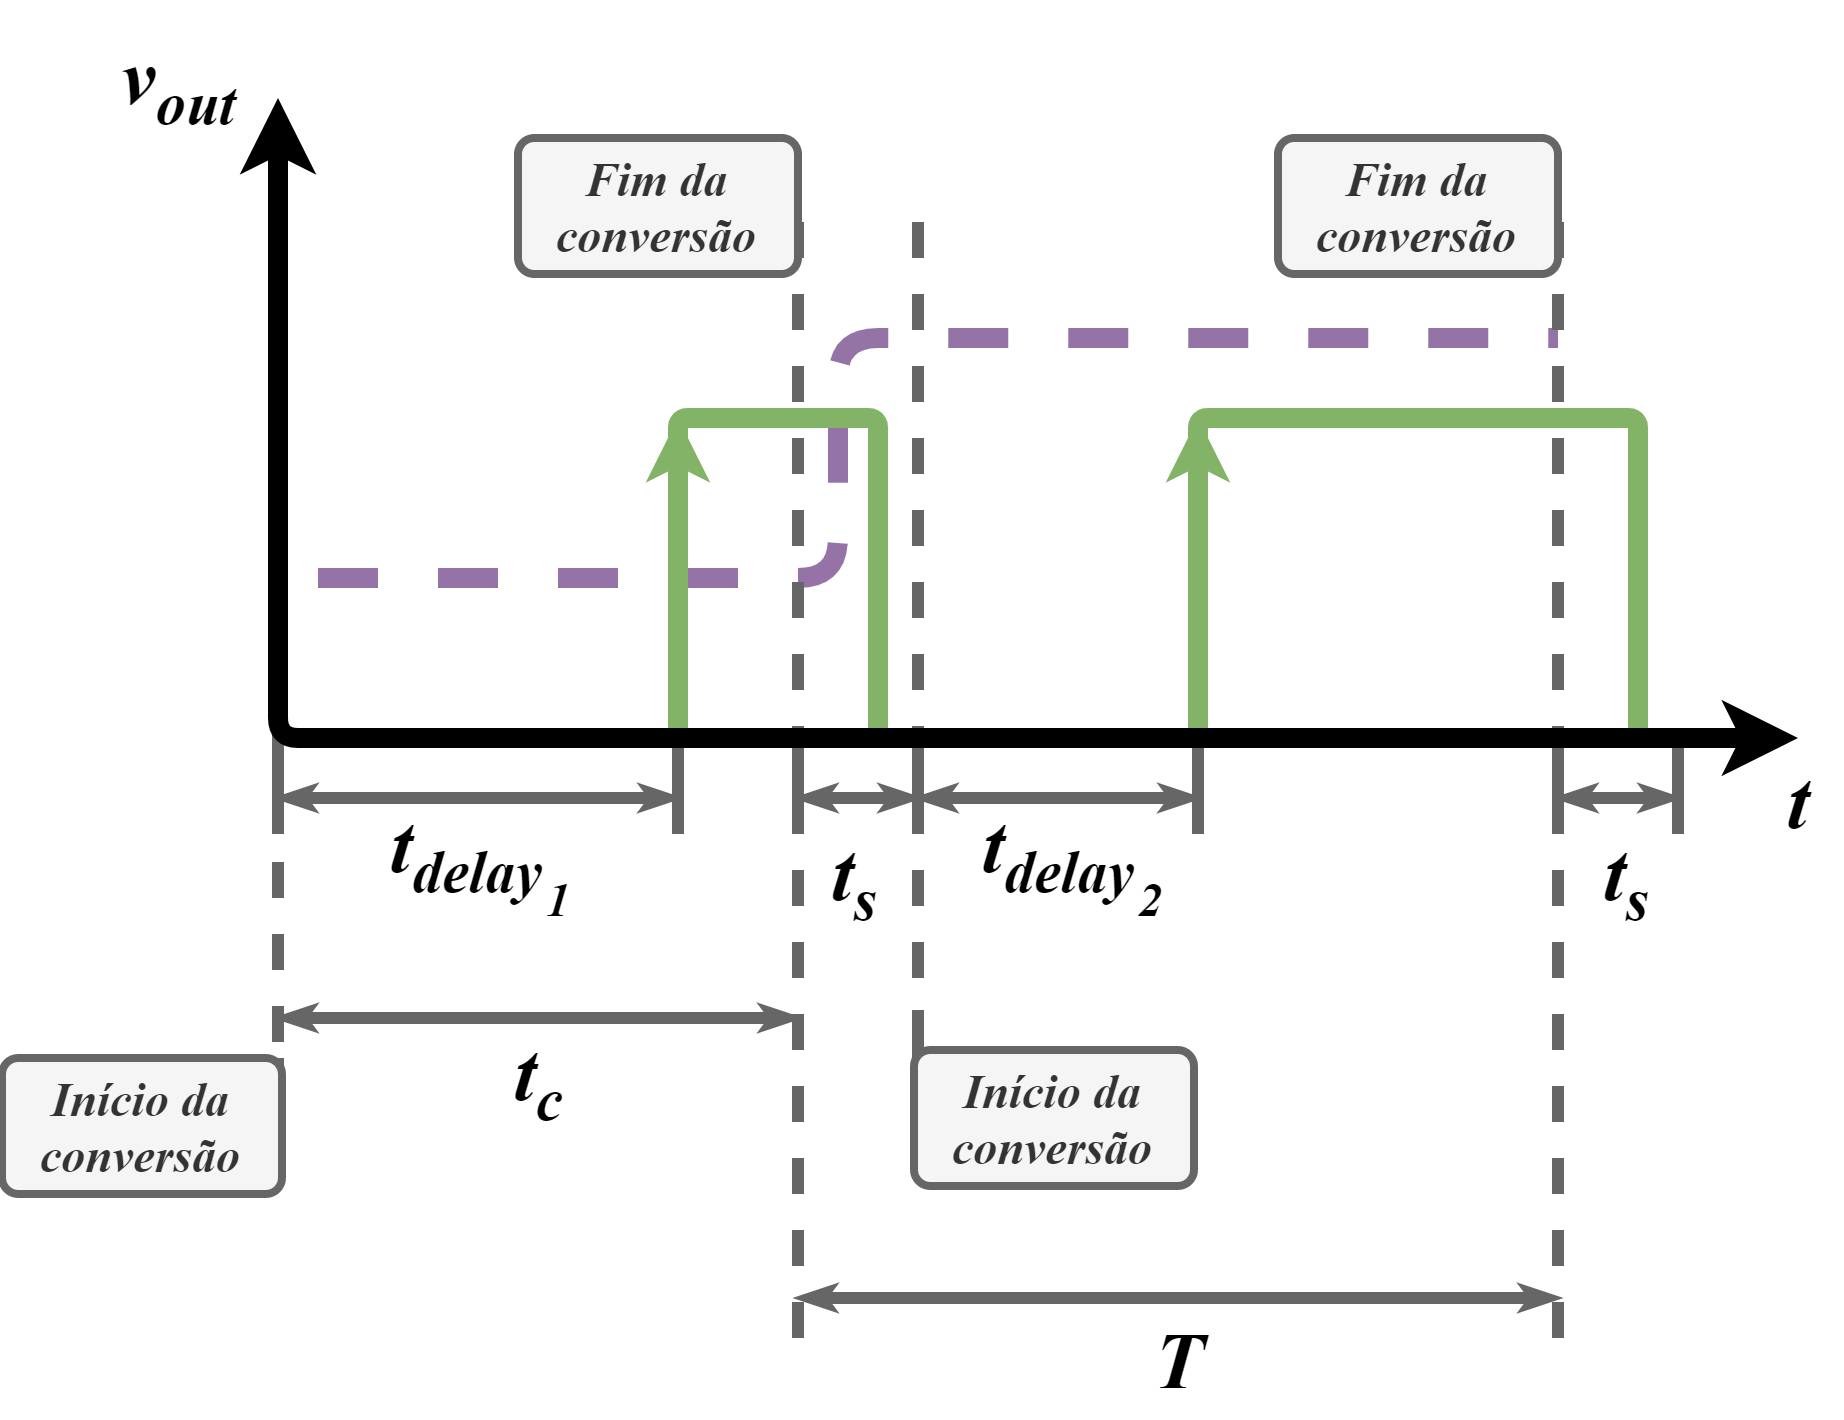
\includegraphics[width=\linewidth/2]{images/time_details.png}
			\caption{Detalhes das definições de tempo do VTC}
			\label{fig:time_details}
		\end{figure}

		\subsection{Princípio de conversão}

			Uma implementação primária de um circuito VTC pode ser vista na Figura~\ref{fig:vtc1}. Esta implementação é denominada unidade de atraso controlada por tensão, ou VCDU\cite{Fei}. O período de amostragem $T$ é controlado pelo sinal $\phi$. O princípio de funcionamento se baseia no chaveamento entre a carga e descarga do capacitor pelo sinal $\phi$ enquanto que a taxa de descarga, e por tanto o tempo $t_{delay}$, é determinado pela amplitude de tensão do sinal $v_{in}$. Os estados de carga e descarga são apresentados nas Figuras~\ref{vtc1_charge} e ~\ref{vtc1_discharge}.

			\begin{figure}[h]
				\centering
				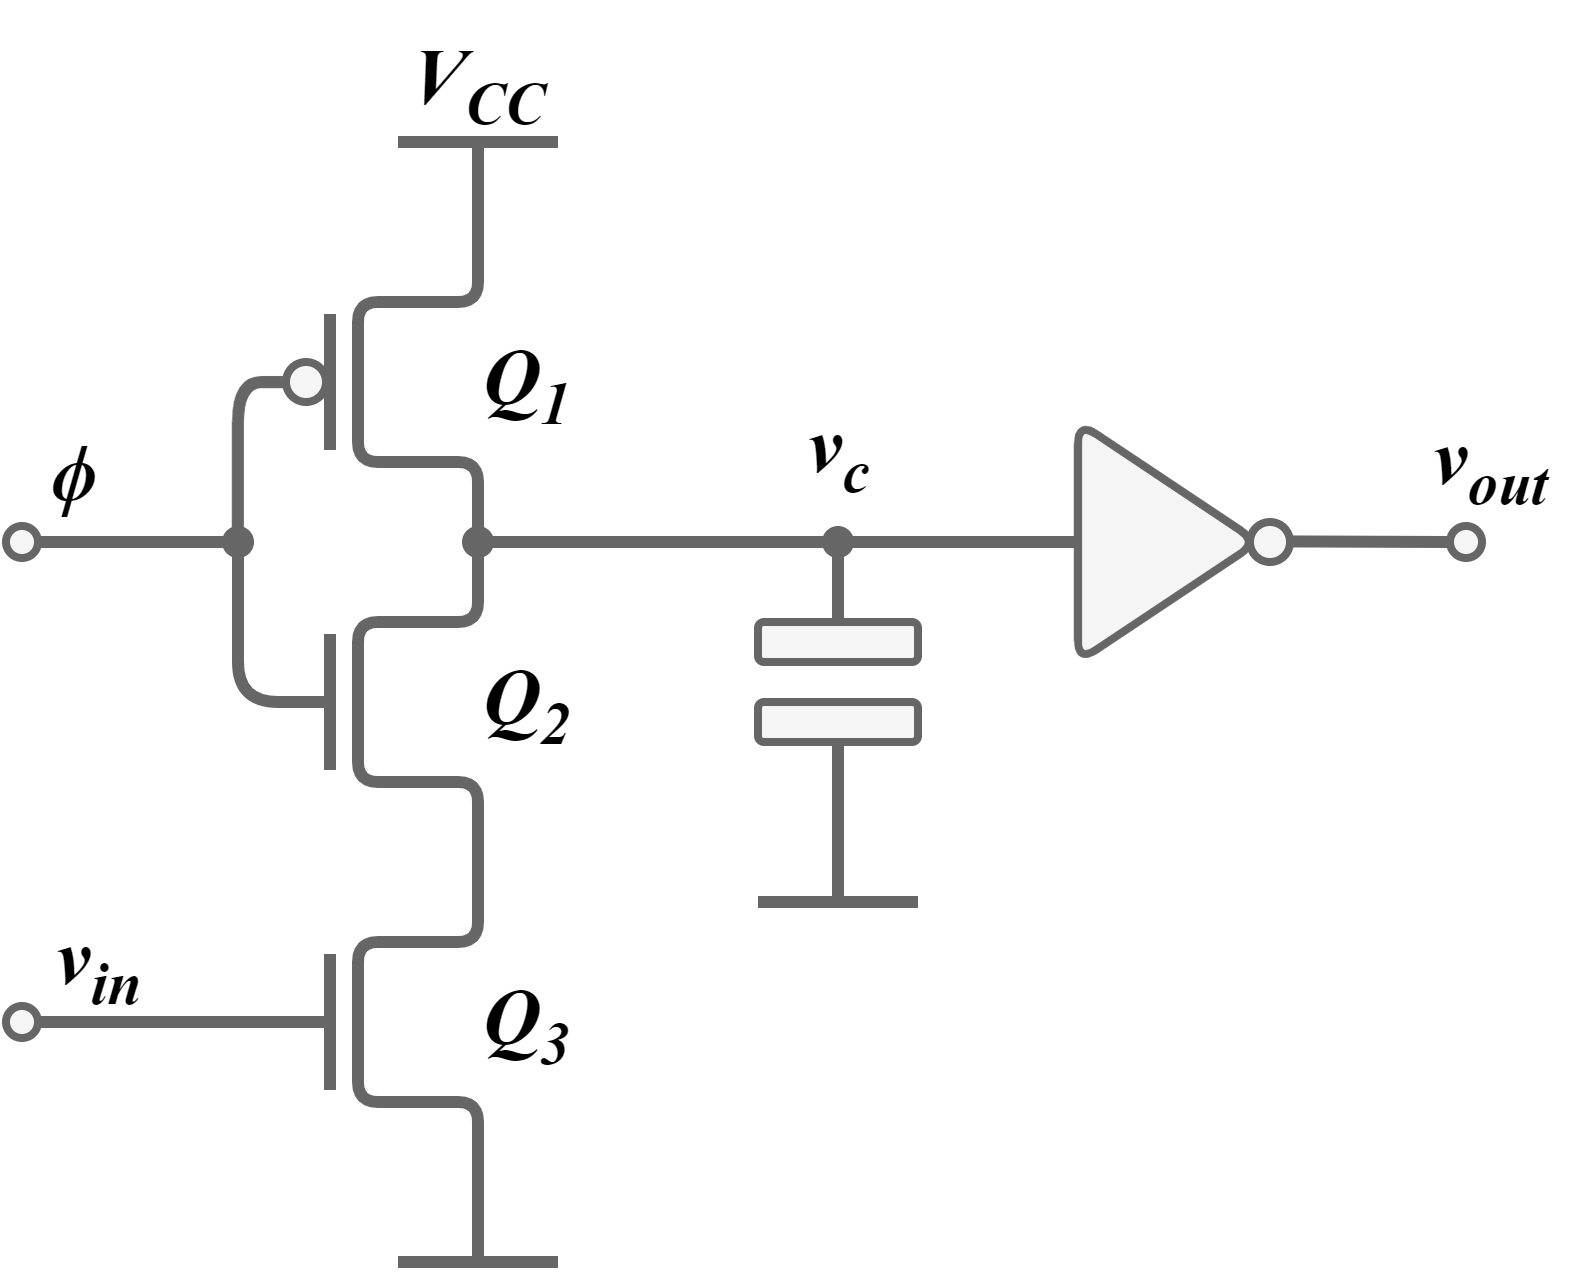
\includegraphics[width=\linewidth/2]{images/VTC_circ1.png}
				\caption{Implementação de um VCDU}
				\label{fig:vtc1}
			\end{figure}

			Quando $\phi$ possui nível de tensão $\phi=0 V$, o capacitor é carregado até a tensão $V_{CC}$ pelo transistor de \textit{pull-up} $Q_1$, como mostrado na figura abaixo. Já quando $\phi$ possui nível de tensão $\phi=V_{CC}$, o capacitor é descarregado pelos transistores $Q_2$ e $Q_3$. O tempo em que $\phi=V_{CC}$ é o que determina o tempo de conversão $t_c$.

			\begin{figure}[!ht]
				\centering
				\begin{minipage}{0.4\linewidth}
					\centering
					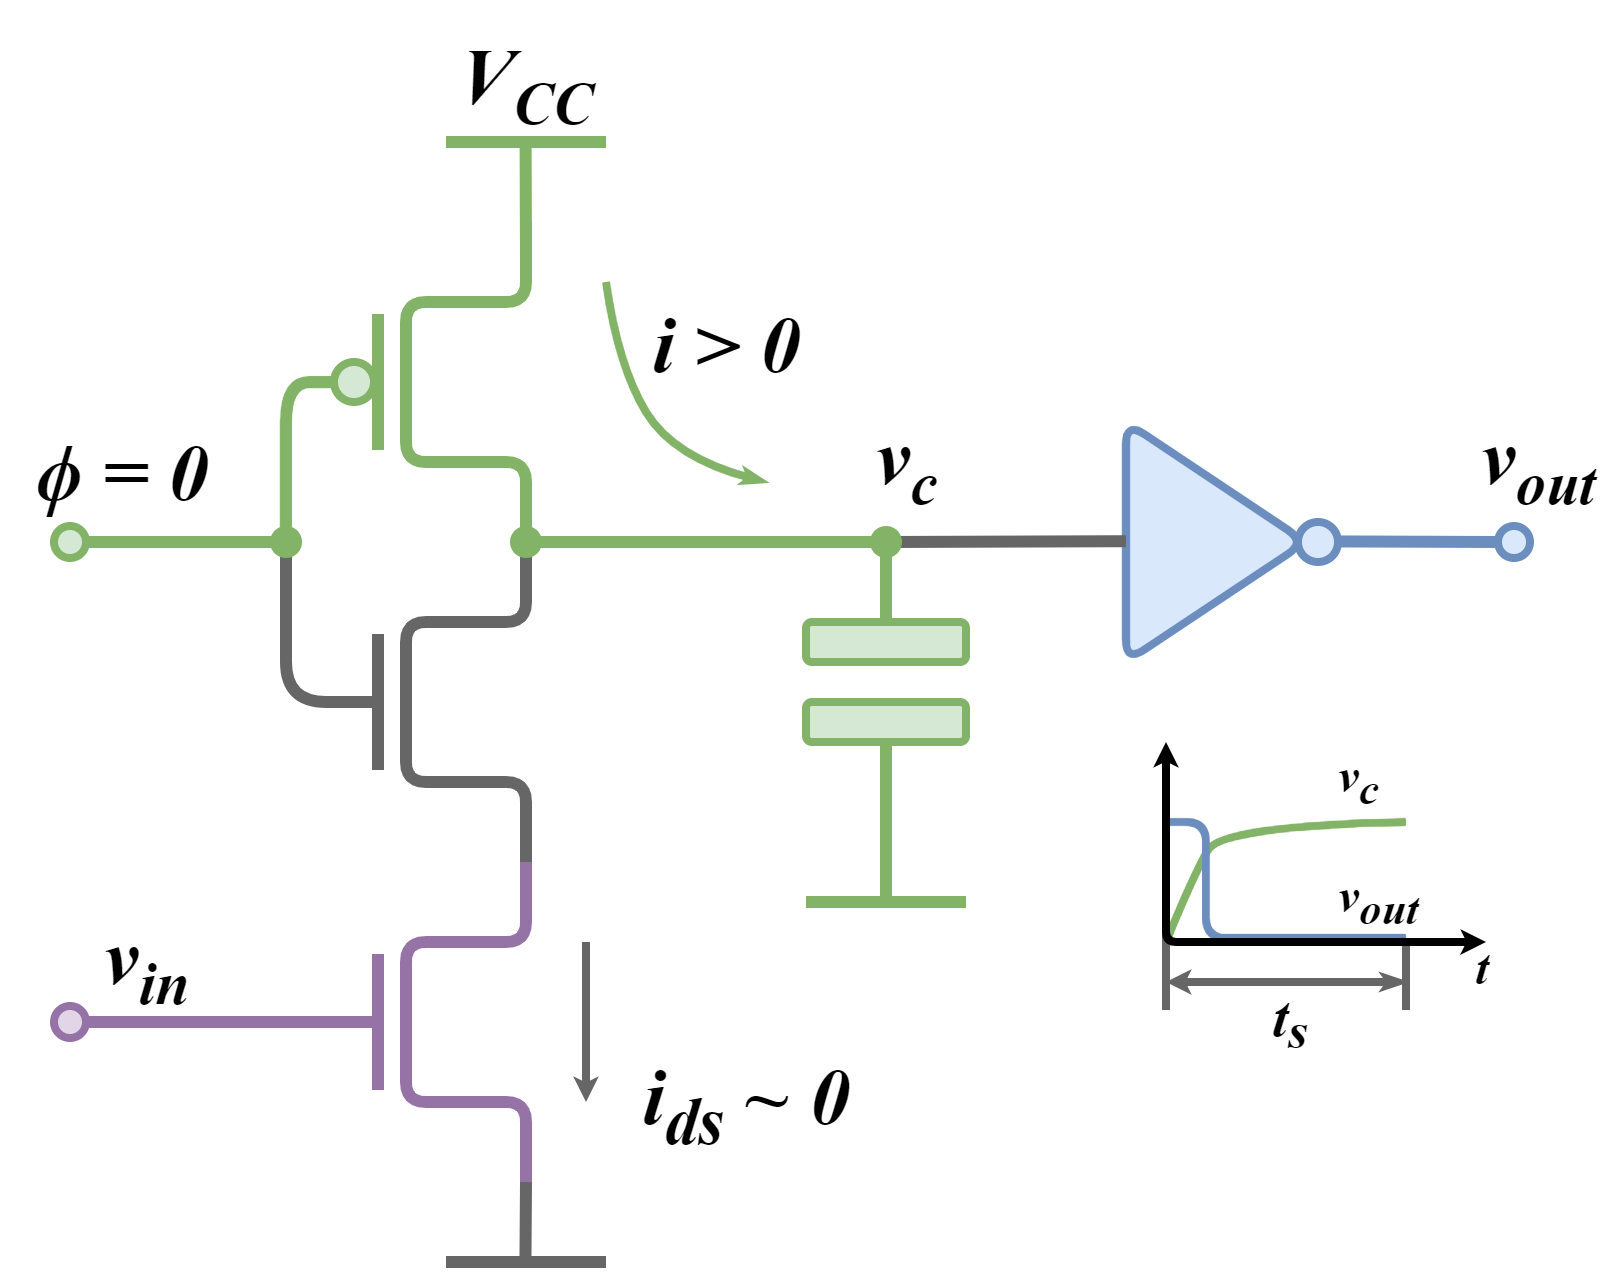
\includegraphics[width = \linewidth]{images/charge.png}
					\caption{VCDU - Carga do capacitor}
					\label{vtc1_charge}
				\end{minipage}
				\hfill\vline\hfill
				\begin{minipage}{0.4\linewidth}
					\centering
					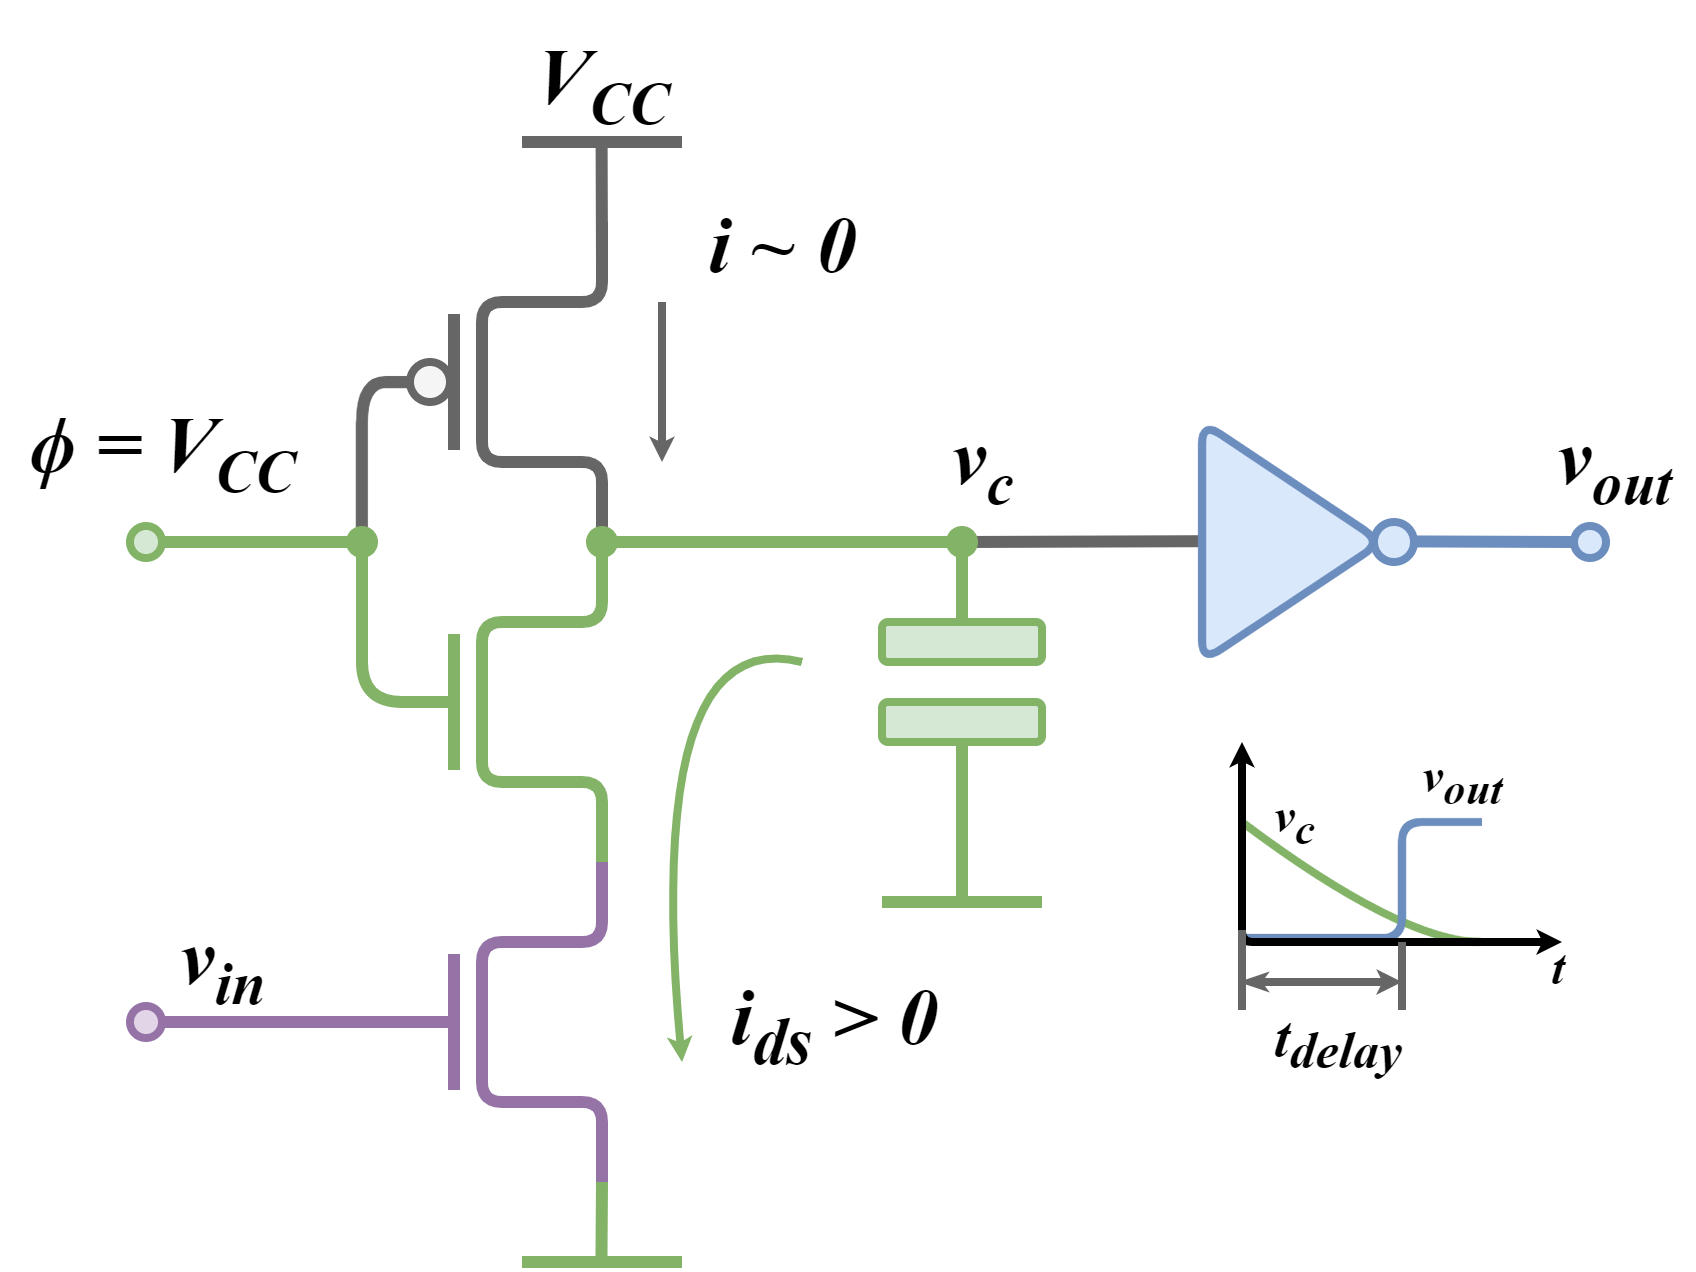
\includegraphics[width = \linewidth]{images/discharge.png}
					\caption{VCDU - Descarga do capacitor}
					\label{vtc1_discharge}
				\end{minipage}
			\end{figure}

			A corrente de descarga $i_{ds}$ é majoritariamente determinada pelo transistor $Q_3$, que por sua vez é proporcional à tensão $v_{in}$. É importante notar que o tempo de carga deve ser menor que o tempo de amostragem $t_s$ e o tempo de descarga deve ser menor que o tempo de conversão $t_c$. O $t_{delay}$ é definido entre o início da descarga e o momento em que a tensão $v_c$ abaixar do valor limiar inferior do inversor de saída, ou seja, a borda de subida de $v_{out}$.

			Uma outra implementação mais refinada de um VTC é o chamado VTC de referência \cite{Fei}, apresentado na Figura ~\ref{fig:vtc2}. O valor de $t_{delay}$ para esse VTC é o intervalo entre a borda  de descida de $\phi$ e quando a tensão no capacitor ultrapassa a tensão $v_{in}$. O princípio de funcionamento é apresentado na Figura ~\ref{vtc2_charge}.

			\begin{figure}[H]
				\centering
				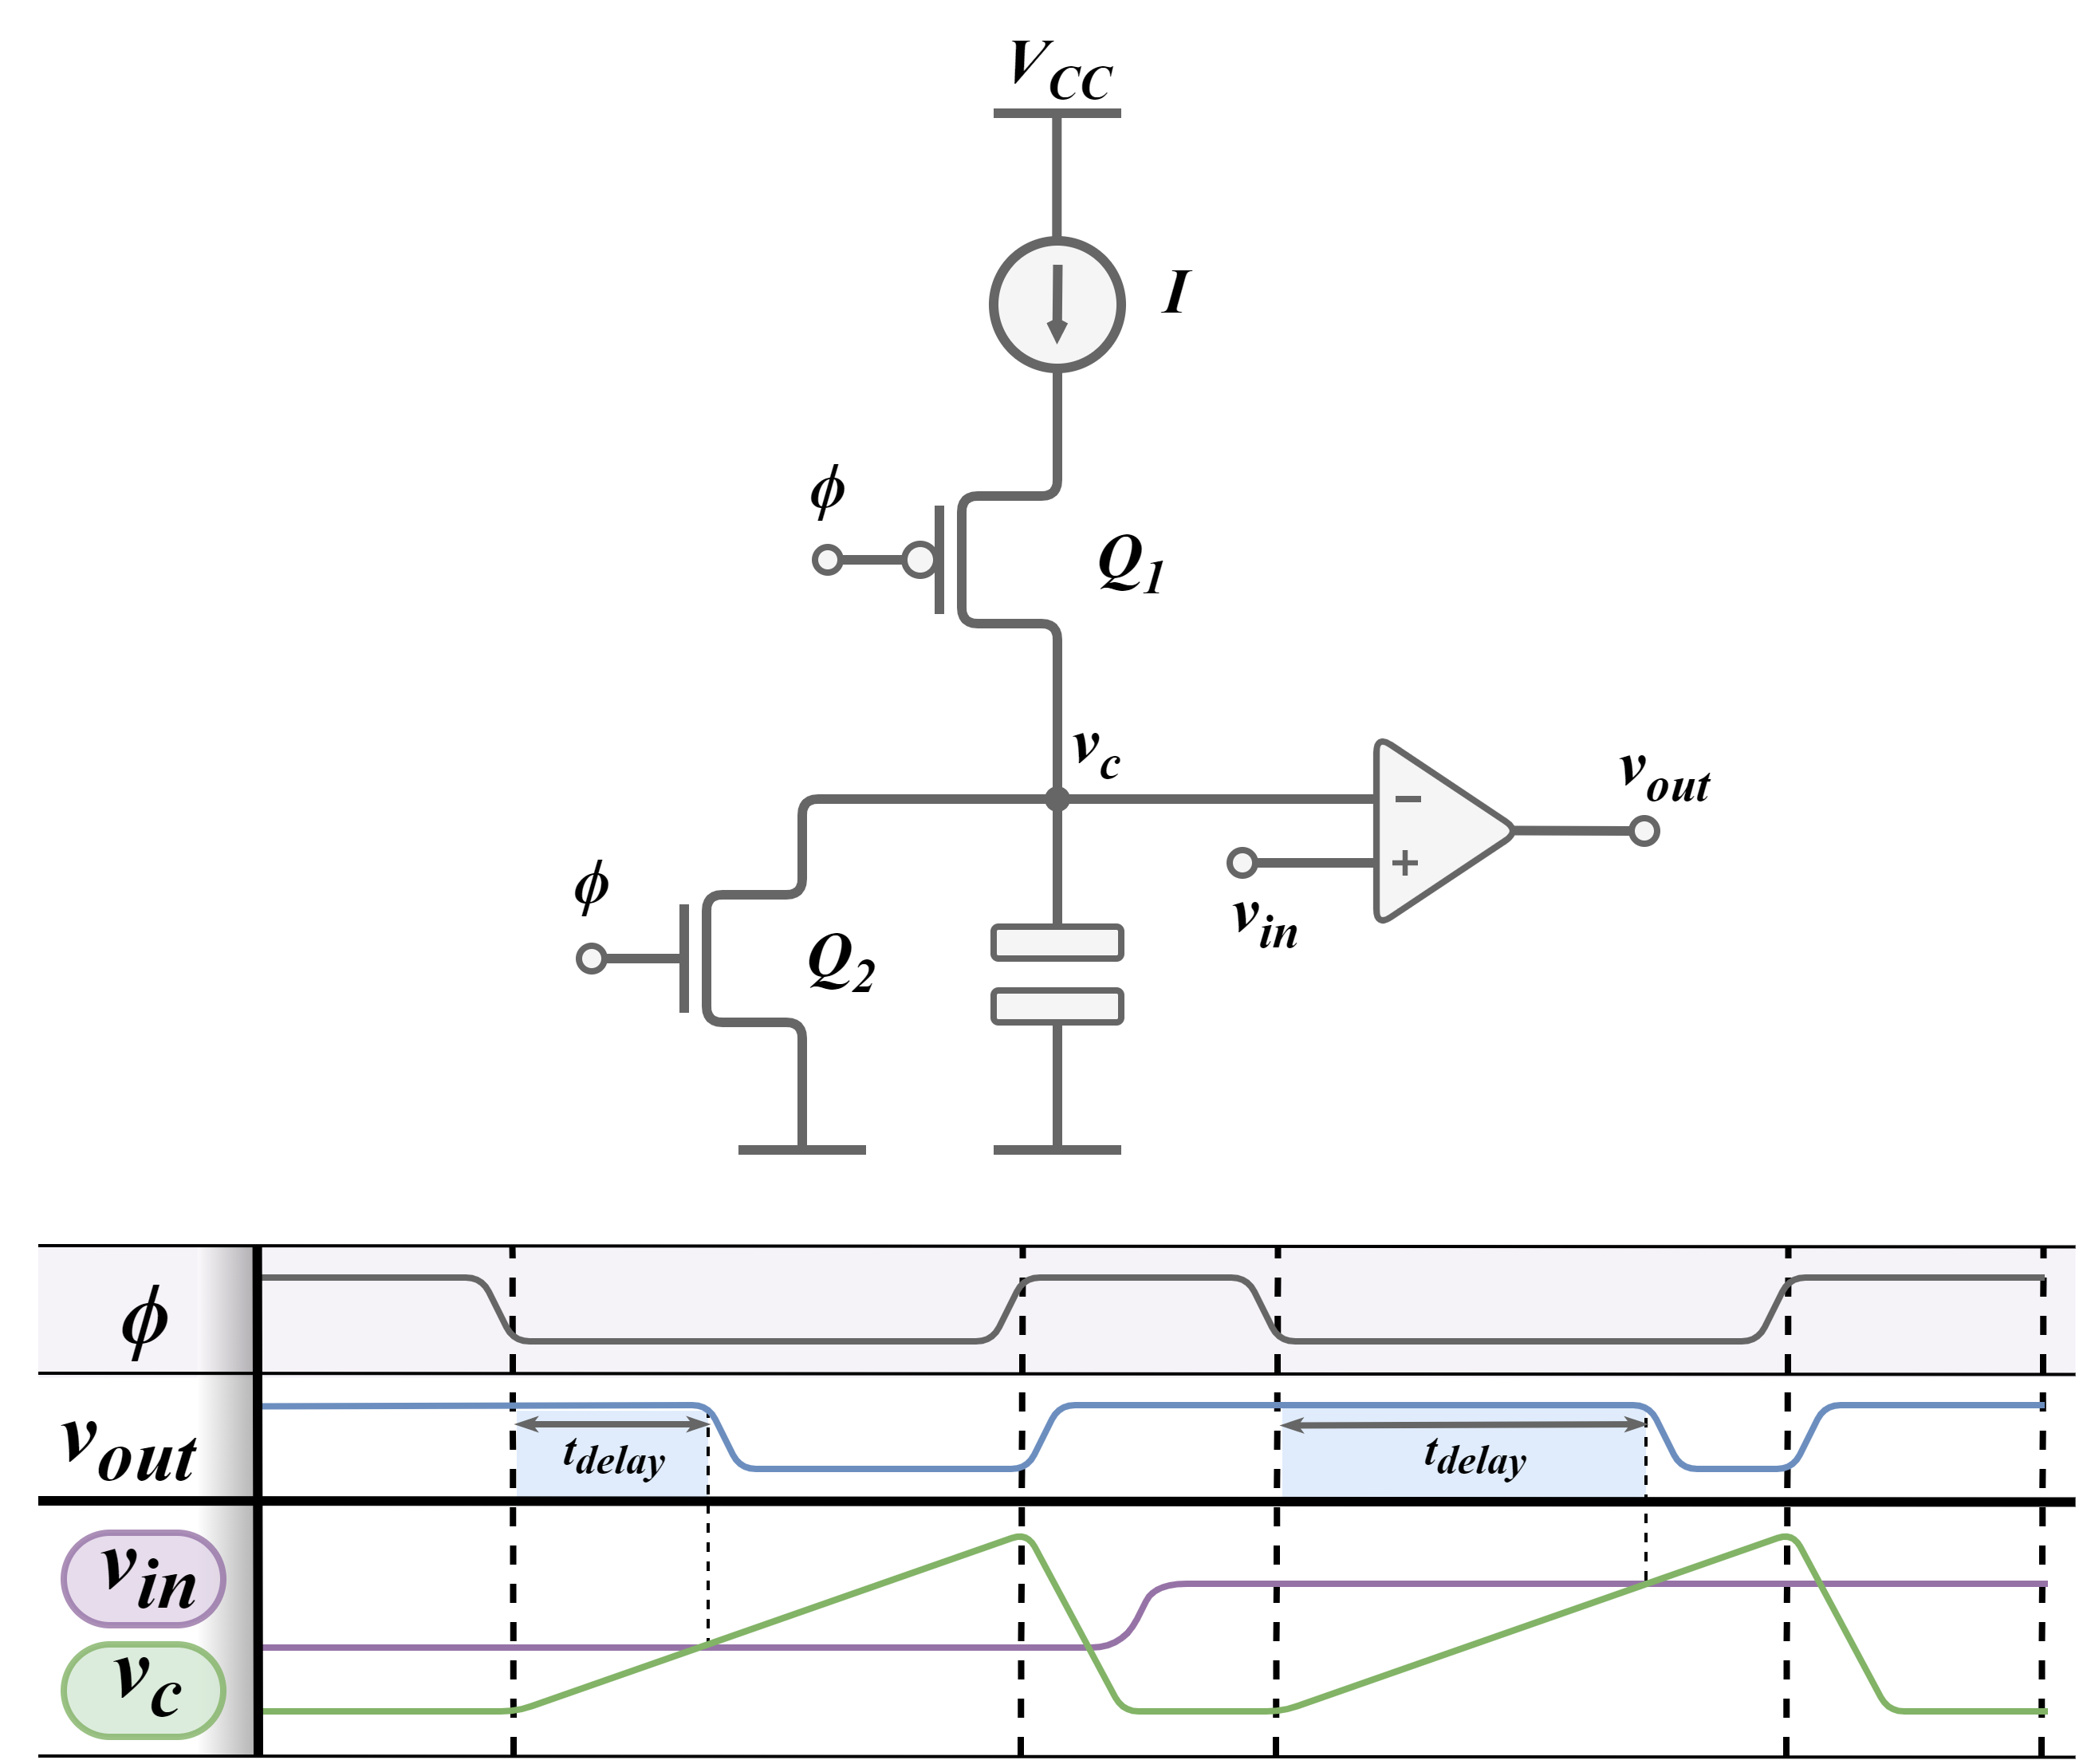
\includegraphics[width=\linewidth*3/4]{images/VTC_circ2.png}
				\caption{VTC de referência}
				\label{fig:vtc2}
			\end{figure}

			O capacitor é carregado por uma fonte de corrente durante a conversão. Quando a tensão do capacitor ultrapassa a tensão $v_{in}$, a tensão $v_{out}=0 V$. Após o ciclo de conversão, o capacitor é descarregado pelo transistor $Q_2$.

			\begin{figure}[h]
				\centering
				\begin{minipage}{0.4\linewidth}
					\centering
					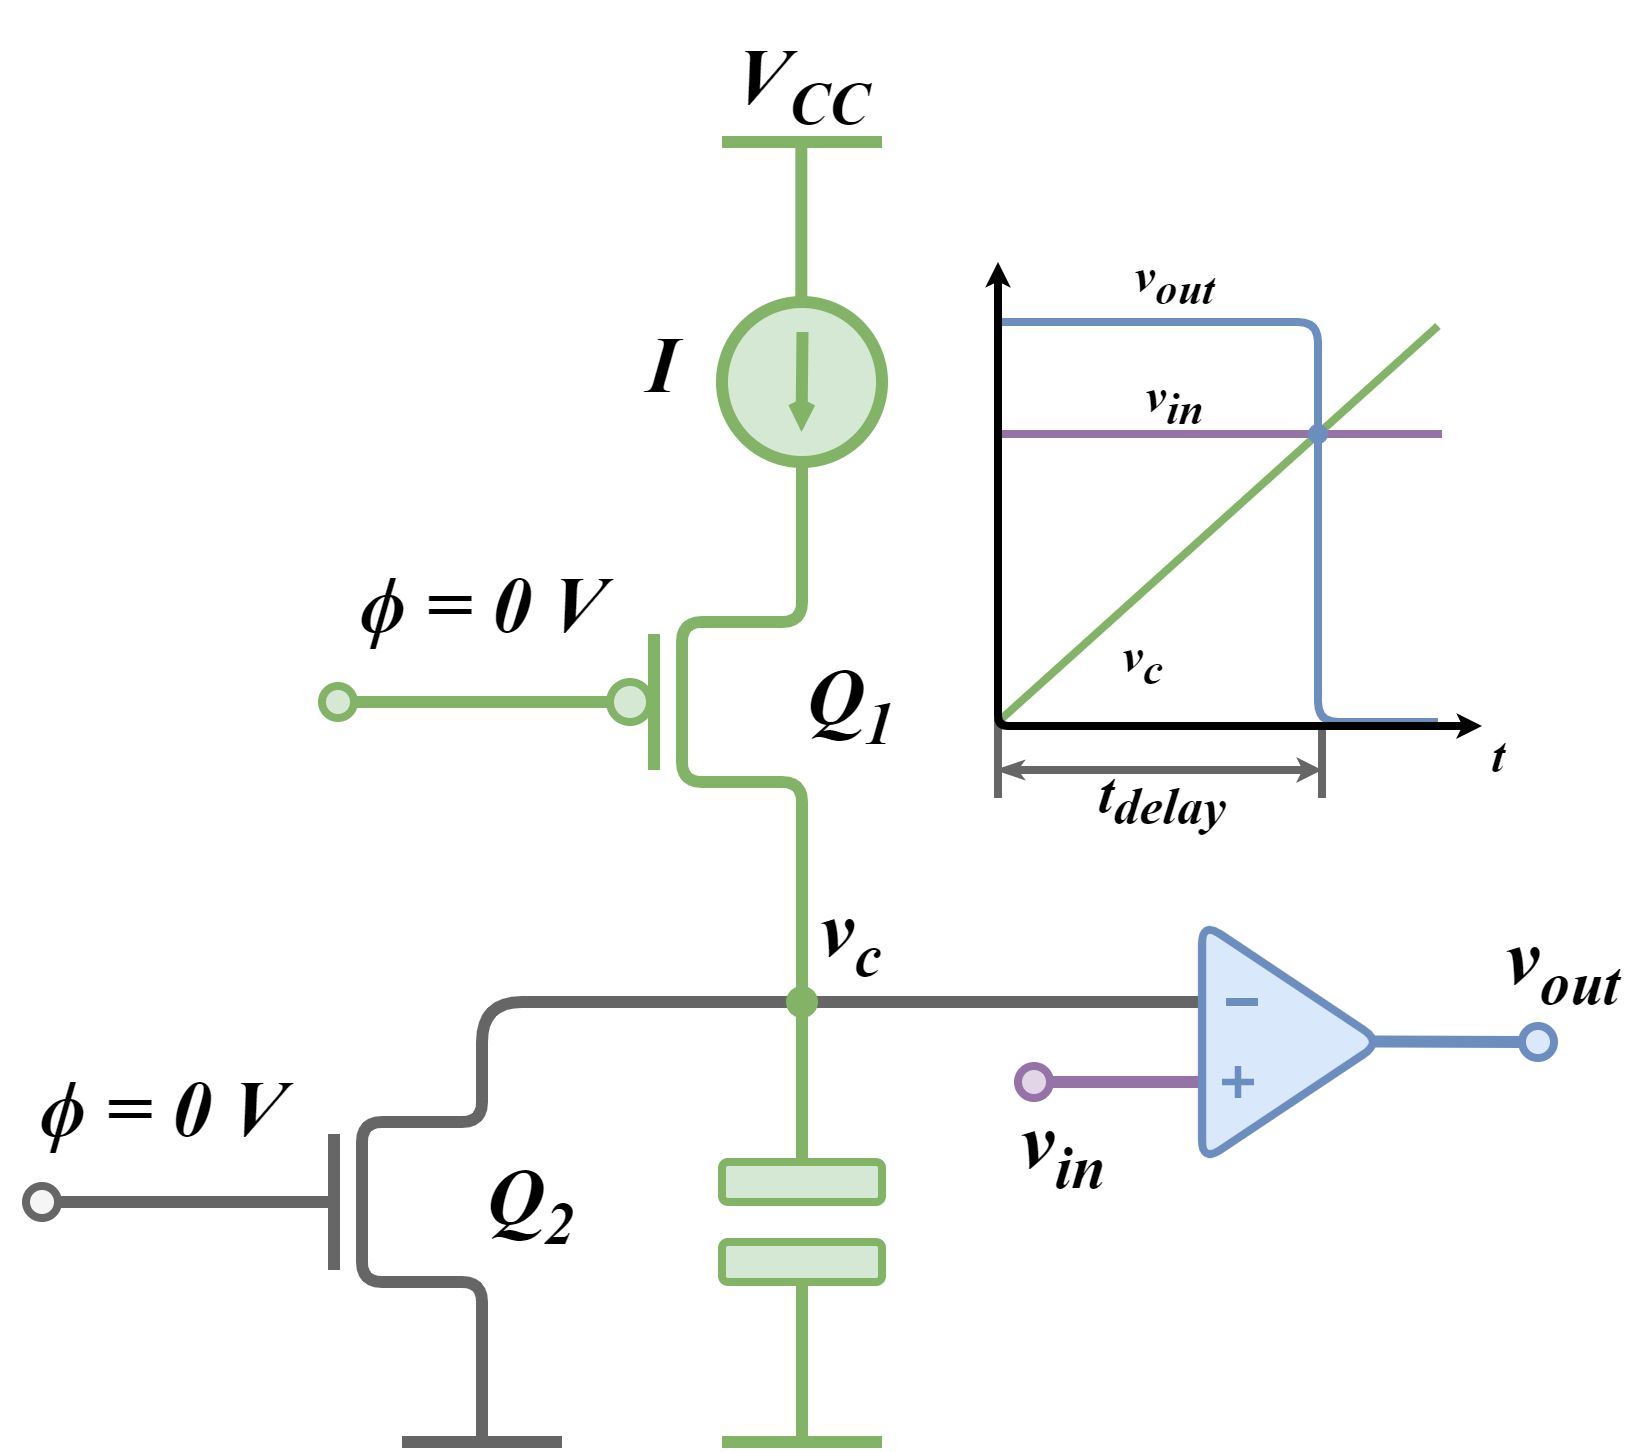
\includegraphics[width = \linewidth]{images/VTC2_charge.png}
					\caption{VTC de referência - Carga do capacitor}
					\label{vtc2_charge}
				\end{minipage}
				\hfill\vline\hfill
				\begin{minipage}{0.4\linewidth}
					\centering
					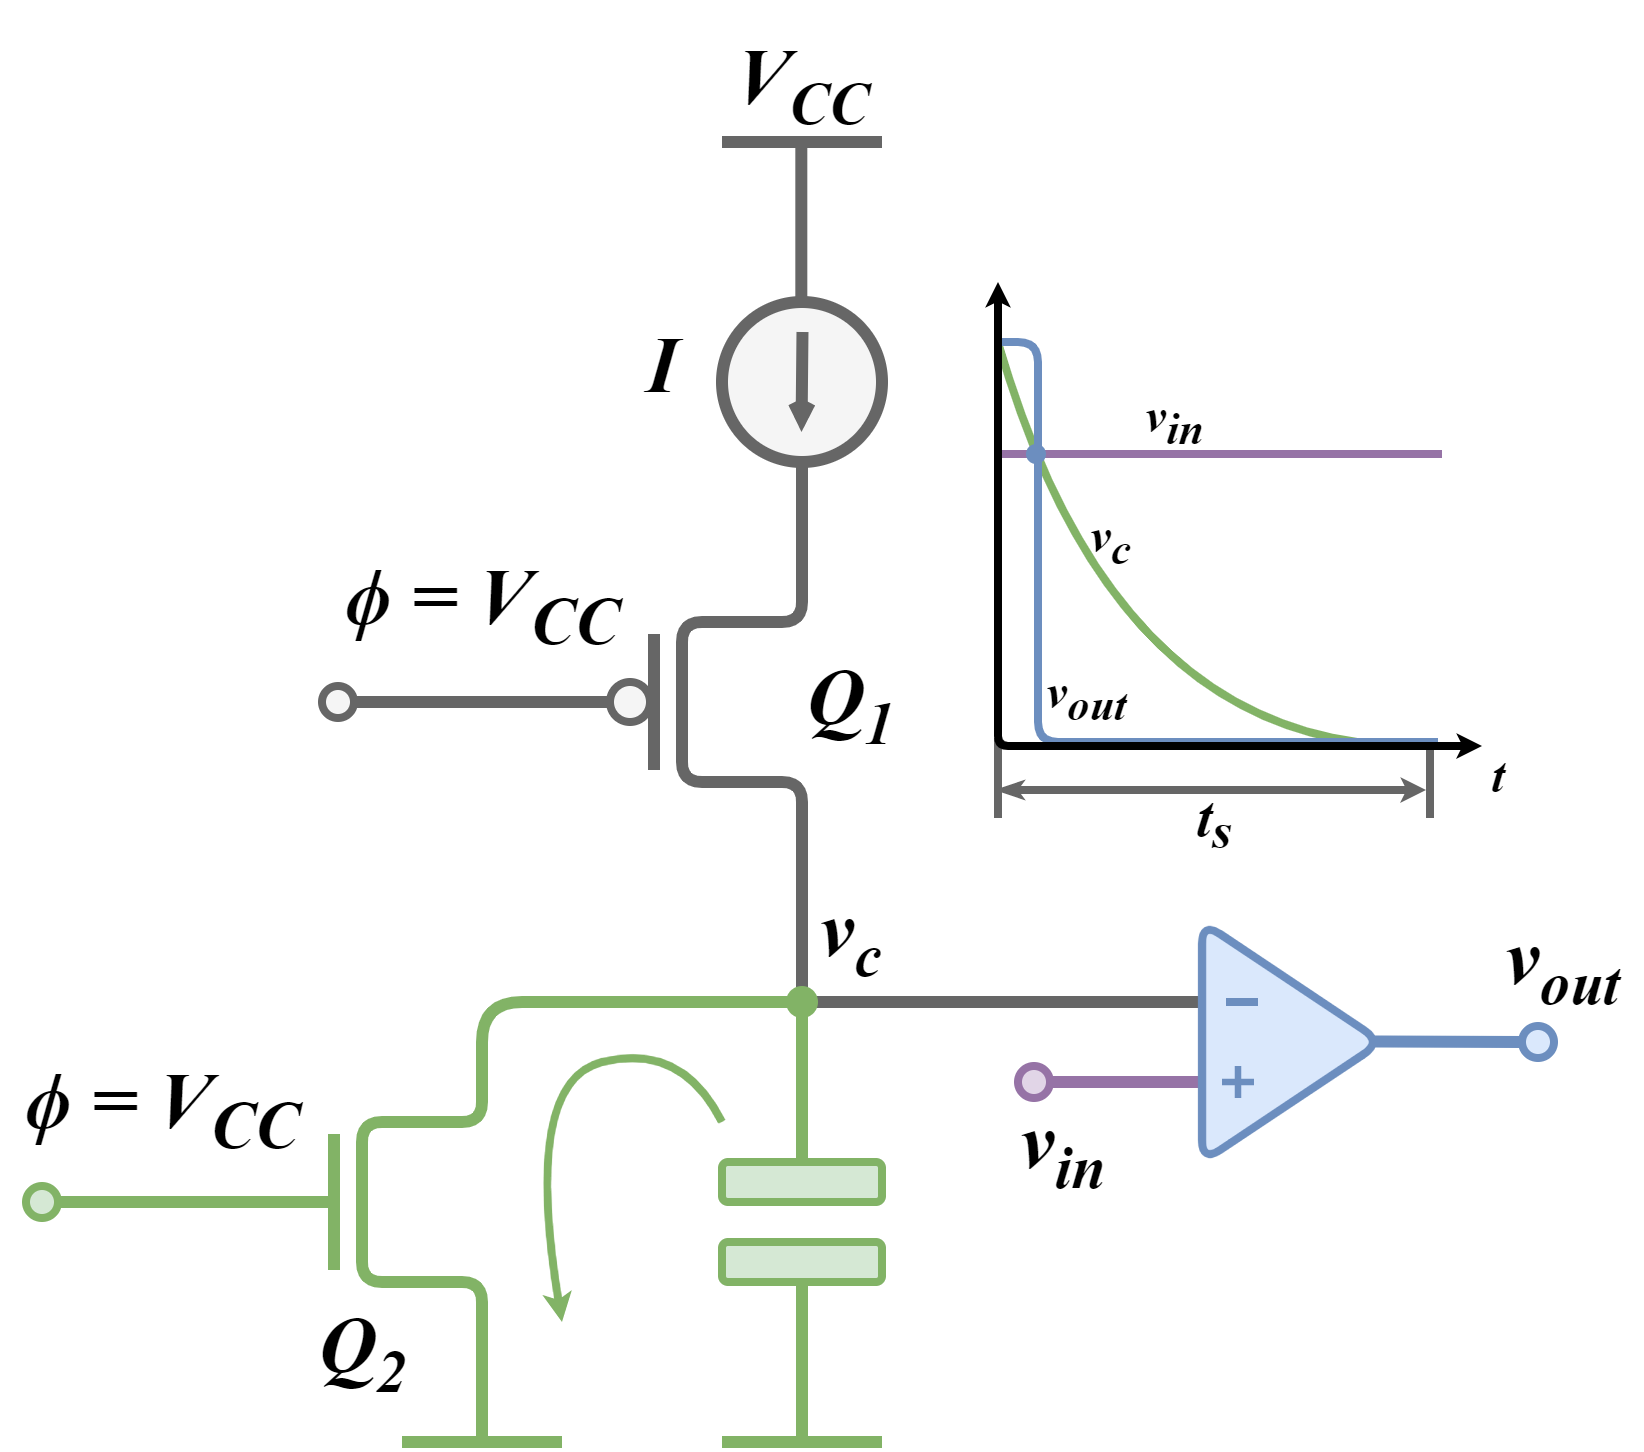
\includegraphics[width = \linewidth]{images/VTC2_discharge.png}
					\caption{VTC de referência - Descarga do capacitor}
					\label{vtc2_discharge}
				\end{minipage}
			\end{figure}

			Há uma gama de implementações de VTCs, cada uma com vantagens e desvantagens que podem ser mais adequadas para cada aplicação. A fim de utilizar métricas para analisar os conversores de tensão para tempo, algumas características podem ser atribuídas aos conversores.

		\subsection{Características dos conversores}


	\section{Conversores tempo-digital}
		Os TDCs quantizam um dado valor $t_{delay}$ em uma representação binária de um ou mais \textit{bits}. Seja um sinal no domínio tempo com valor $t_{delay}$
			

	% \section{Conversor analógico-digital}
	% 	O conversor analógico-digital, ou ADC, é responsável por digitalizar um analógico. A conversão é referenciada às tensões de alimentação do ADC  graduada de acordo com o número de \textit{bits} \cite{artElectronics}. 
		
	% 	Como exemplo, um conversor alimentado por uma tensão de $5 V$ e com $10$ \textit{bits} de resolução possui $2^{10}$ divisões. Assim, a menor divisão do conversor é de $5/2^{10} = 4,88 mV$ e, consequentemente, esse é o menor valor que pode ser detectado pelo ADC. Se a resolução fosse de $12$ \textit{bits} ao invés de $10$ \textit{bits}, a resolução do conversor seria de $5/2^{12}=1,22 mV$. Esse também é o passo do conversor, também definido como LSB (\textit{Least Significant Bit}), ou seja, todas os valores digitalizados são múltiplos da resolução.
%#Endregion

% ----------------------------------------------------------
%#Region Capítulo 3 - Materiais, Métodos e Desenvolvimento
% ----------------------------------------------------------
% \chapter{Materiais, Métodos e Desenvolvimento}
	
%#Endregion

% ----------------------------------------------------------
%#Region Capítulo 4 - Resultados
% ----------------------------------------------------------
% \chapter{Resultados}

%#Endregion

% ----------------------------------------------------------
%#Region Capítulo 5 - Conclusões
% ----------------------------------------------------------
% \chapter{Conclusões}

%#Endregion

% ---
% Finaliza a parte no bookmark do PDF, para que se inicie o bookmark na raiz
% ---
\bookmarksetup{startatroot}% 
% ---

% ----------------------------------------------------------
% ELEMENTOS PÓS-TEXTUAIS
% ----------------------------------------------------------
\postextual

% ----------------------------------------------------------
% Referências bibliográficas
% ----------------------------------------------------------
% \bibliography{abntex2-modelo-references}
\bibliography{bibliografia}

% ----------------------------------------------------------
% Apêndices
% ----------------------------------------------------------

% % ---
% % Inicia os apêndices
% % ---
% \begin{apendicesenv}

% % Imprime uma página indicando o início dos apêndices
% \partapendices

% % ----------------------------------------------------------
% \chapter{A}
% % ----------------------------------------------------------

% % ----------------------------------------------------------
% \chapter{B}
% % ----------------------------------------------------------
% \label{ape:calculoCorrente}

% \end{apendicesenv}
% % ---

% ----------------------------------------------------------
% Anexos
% ----------------------------------------------------------

% ---
% Inicia os anexos
% ---
% \begin{anexosenv}

% % Imprime uma página indicando o início dos anexos
% \partanexos

% % ---
% \chapter{Morbi ultrices rutrum lorem}
% % ---
% %\lipsum[60]

% % ---
% \chapter{Cras non urna sed feugiat cum sociis natoque penatibus}
% % ---
% %\lipsum[61-63]

% % ---
% \chapter{Fusce facilisis lacinia dui}
% ---
%\lipsum[64-65]

% \end{anexosenv}

\end{document}
